\chapter{Grundlagen}
\label{ch:Grundlagen}

In diesem Kapitel werden die verwendeten Technologien kurz erklärt und begründet, warum sie für diese Arbeit eine Bedeutung haben. Außerdem werden grundlegende Entscheidungen herbeigeführt, auf die sich die weitere Arbeit stützt.

\section{Häufigkeit der Richtungsänderung}
In Bezug auf die Rechtzeitigkeit der Steuerung ist es wichtig, dass für den Nutzer keine Verzögerungserscheinungen bei der Richtungsänderung des Roboters auftreten. Da der Mensch eine gewisse Latenz aufweist, um von der Analyse des Geschehens eine Handlung zu tätigen, hat die minimal notwendige Frequenz für Richtungsänderungen hier etwas Spielraum. Nach einigen Testläufen hat sich herausgestellt, dass eine Befehlsfrequenz von 10Hz ausreichend ist, um die Rechtzeitigkeit zu gewährleisten. Die maximale Verzögerung von der Initiierung bis zur Umsetzung der Richtungsänderung beträgt hierbei maximal 100ms. Auch die Statusnachrichten kommen in diesem Intervall, es sei denn, es werden noch Bilddaten angehängt. In diesem Fall sendet der Roboter ohne Pausen zwischen den Paketen, damit die Bilddaten möglichst verzögerungsfrei auf dem Steuergerät angezeigt werden können. 


\section{Wahl der Endgeräte für die Steuercontroller}
\label{sec:wahl_endgeraete}
Für die Wahl der Endgeräte kamen einige Komponenten in Frage. Für die meisten Personen ist heutzutage ein Smartphone der ständige Wegbegleiter. Deshalb bietet es sich an die Steuerung über ein Smartphone zu realisieren. Jedoch gibt es Unterschiede zwischen den verschiedenen Betriebssystemen der Smartphones. Die am weitesten verbreiteten sind Android und iOS. Der Nachteil von iOS liegt darin, dass die Entwicklung in einer von Apple eigens entwickelten Programmiersprache stattfindet. Android basiert auf Java und ist deshalb leichter anzuwenden. \\
Um ein breiteres Nutzerspektrum abzudecken soll zusätzlich eine Webanwendung entwickelt werden, um die Roboter mithilfe von Laptops oder PCs zu steuern. 


\section{UDP}
Beim User Datagram Protocol handelt es sich um ein verbindungsloses und in jeglicher Hinsicht ungeschütztes Protokoll, das auf der Transportebene (Schicht 4 im OSI-Schichtenmodell) arbeitet. Es bestehen keinerlei Mechanismen, die das korrekte Übertragen von Paketen gewährleisten. 

\begin{figure}[h]
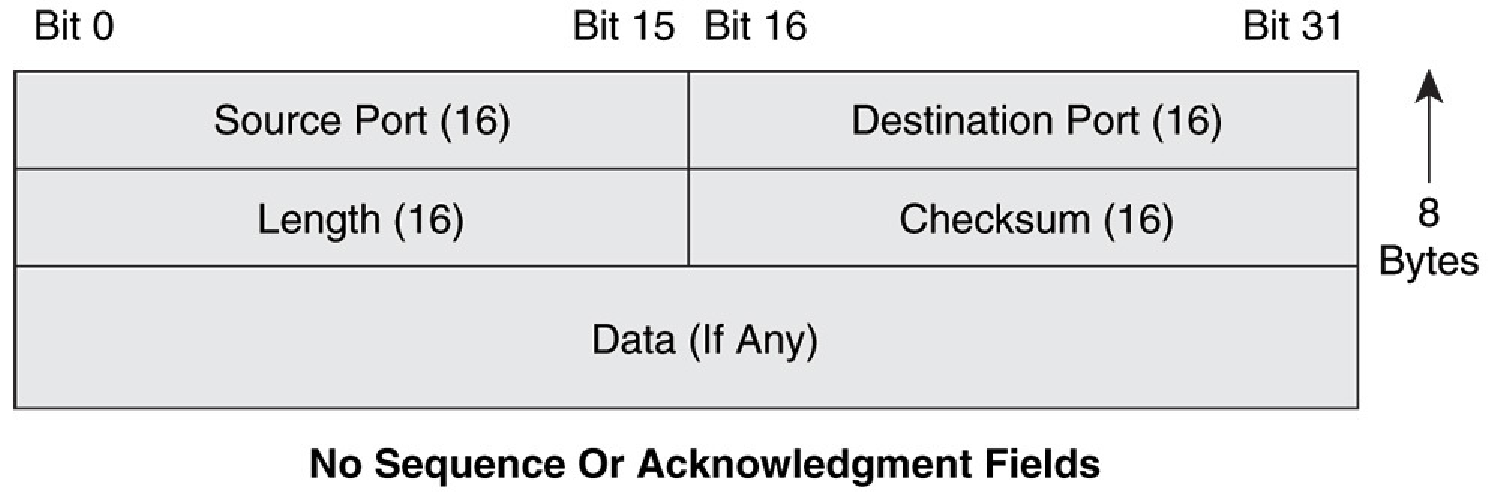
\includegraphics[width=\textwidth]{images/UDP_header.pdf}
\caption{UDP Header}
\label{fig:udp_header}
\end{figure}

Ein UDP Header besteht aus 8 Byte. Mit diesen 8 Byte werden lediglich Source-Port, Destination-Port, Länge und die Checksumme übertragen. Dieser vergleichsweise kleine Header (vgl. TCP mit etwa 20 Byte), führt zu einem geringen Overhead während der Übertragung, auch bei kleinen Paketen. Nachdem ein Paket gesendet wurde erfolgt keine Bestätigung des Pakets vom Empfänger. Durch diesen Uni-Direktionalen Sendevorgang entsteht wenig Traffic im Netzwerk. Falls gewisse Sicherheitsmechanismen gewünscht sind, müssen diese in höheren Schichten implementiert werden. \\
Aufgrund dieser Eigenschaften wird UDP in Bereichen eingesetzt, in denen es auf hohe Übertragungsgeschwindigkeit ankommt und eventuelle Paketverluste zu verkraften sind, bzw. von höheren Schichten aufgelöst werden.\\

Bei der Kommunikation mit dem Roboter kommt es hauptsächlich auf die Geschwindigkeit der Übertragung an. Einzelne Paketverluste sind vertretbar, da das fehlende Paket von dem nächsten ankommenden Paket ersetzt wird. Deshalb ist UDP hierfür das richtige Protokoll.


\section{TCP}
Beim Transmission Control Protocol handelt es sich um ein verbindungsorientiertes paketvermittelndes Protokoll. Mithilfe verschiedener Mechanismen wird sichergestellt, dass Pakete in der richtigen Reihenfolge ankommen, es zu keinen Staus kommt und dass Netzwerkknoten nicht überlaufen. Dadurch, dass das Protokoll verbindungsorientiert arbeitet, können beide Teilnehmer der Verbindung Daten ohne Anfragen senden. 

\begin{figure}[h]
	\centering
	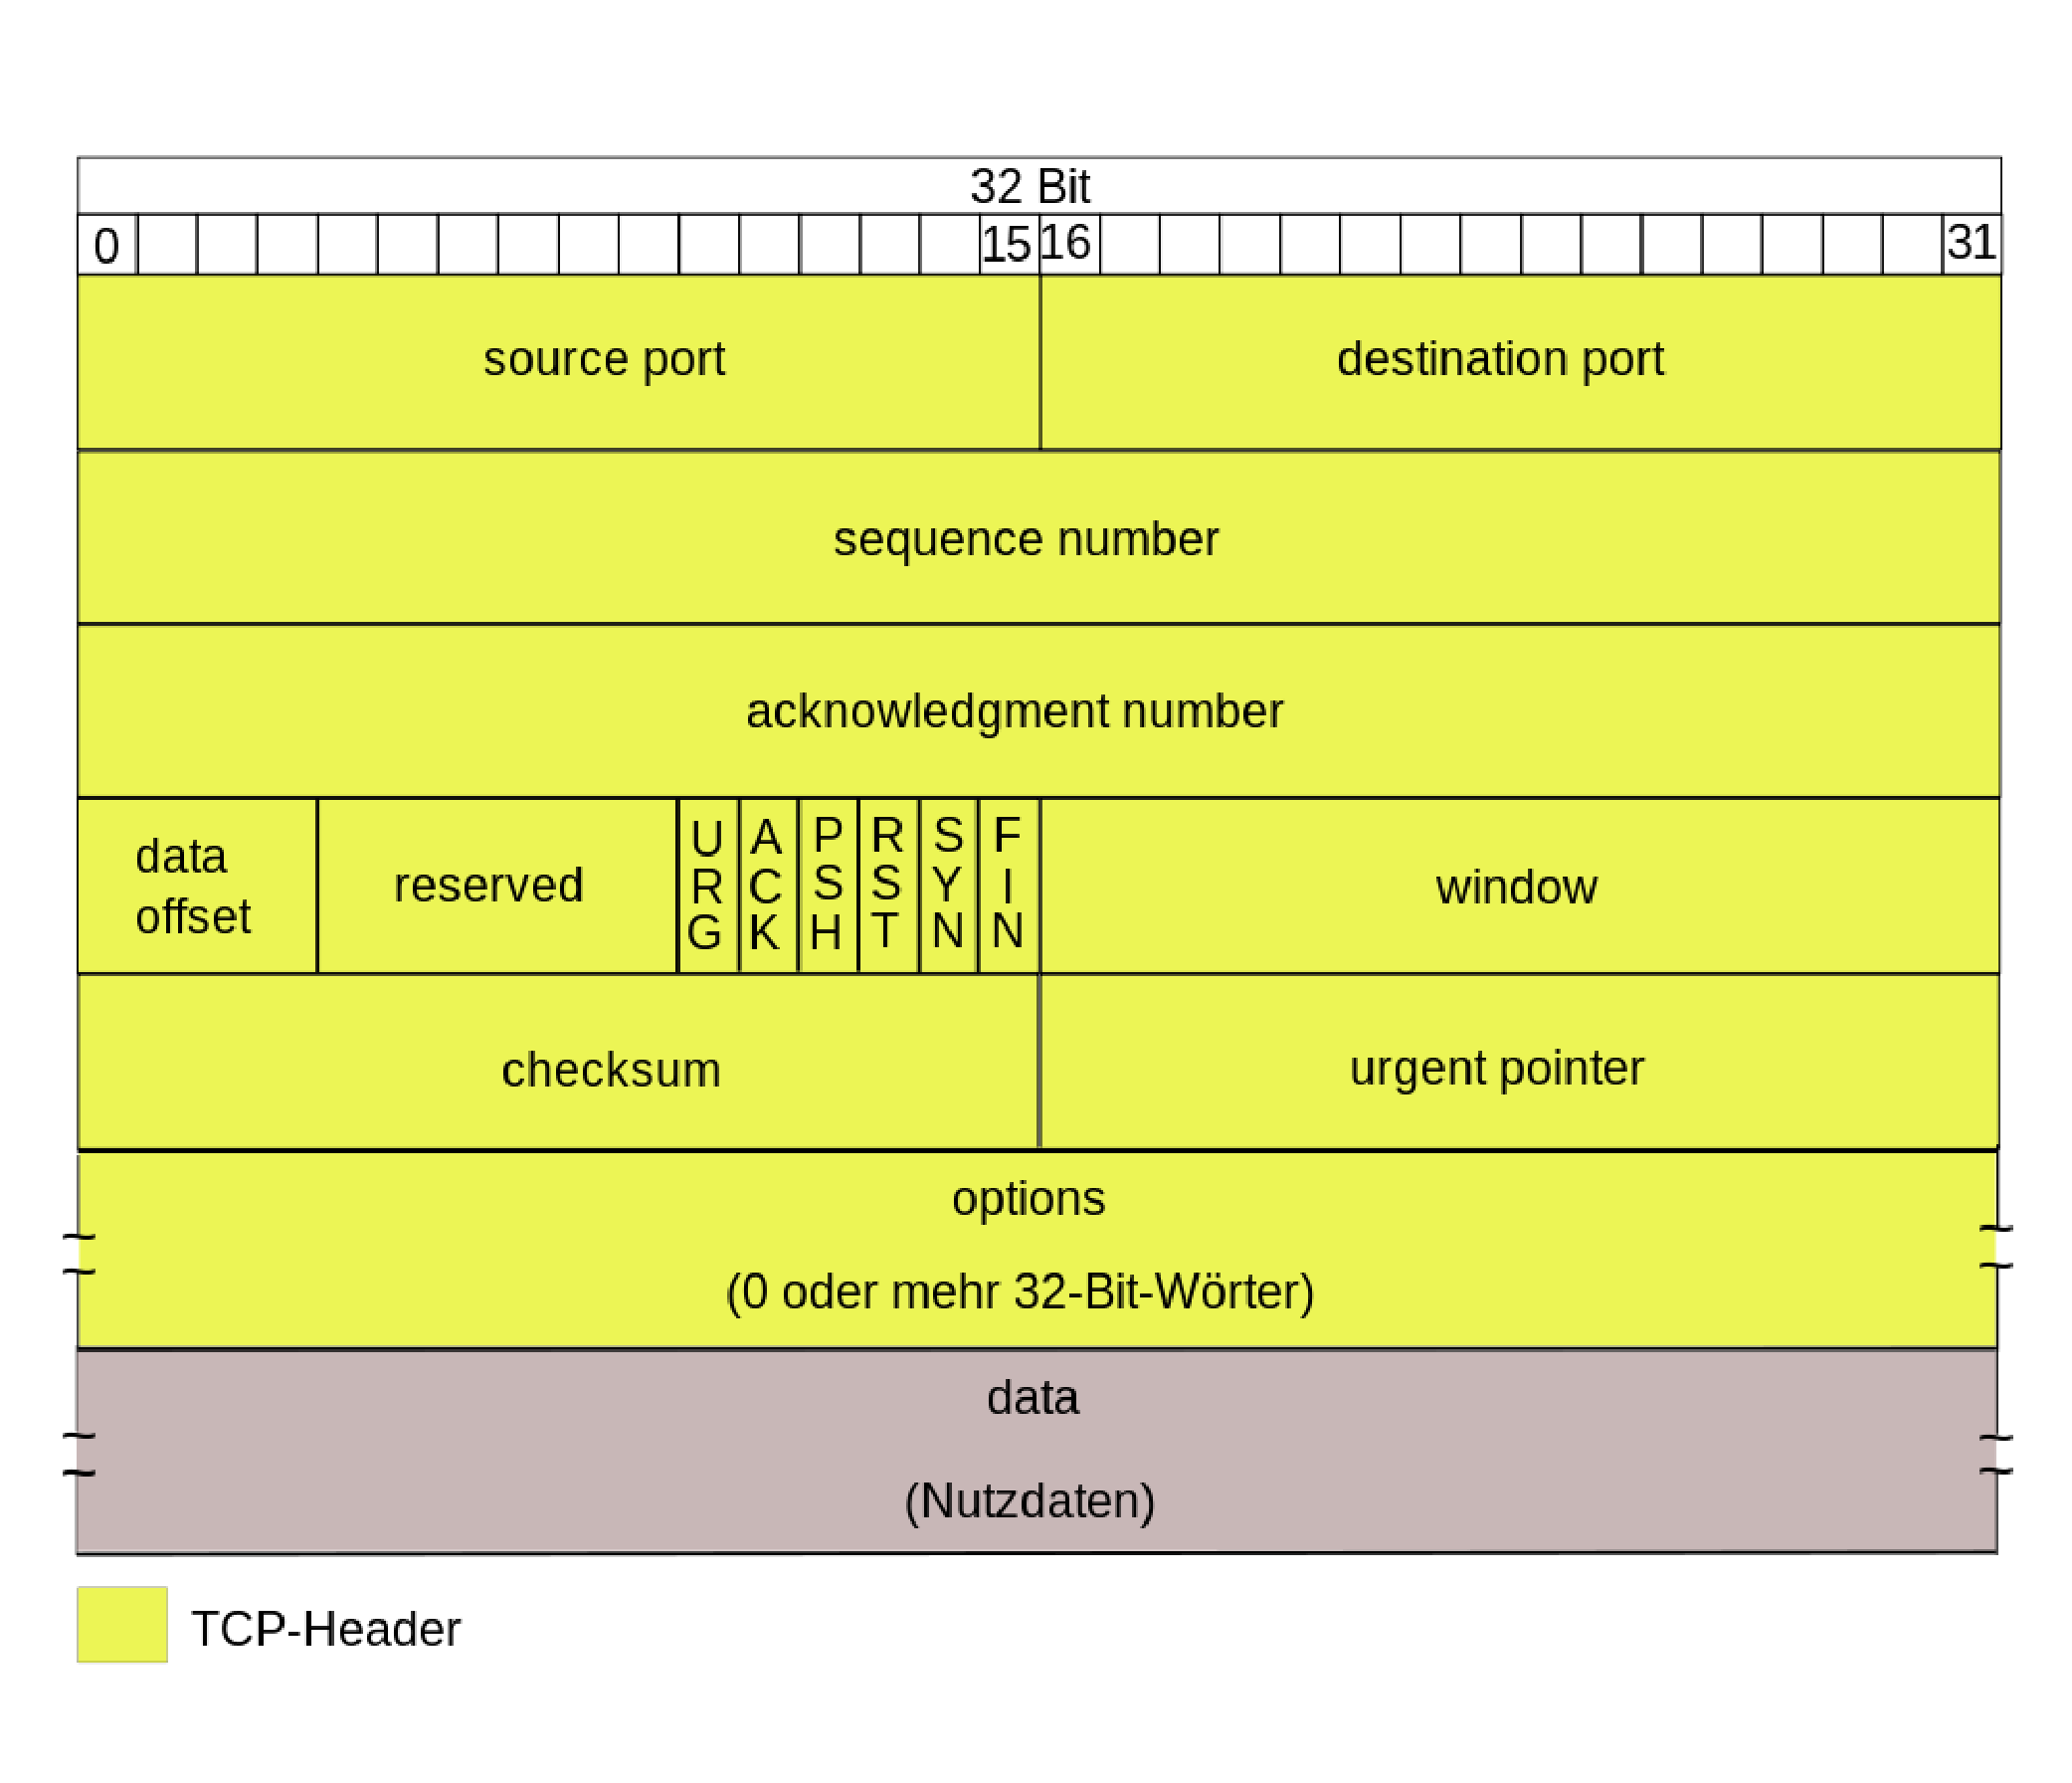
\includegraphics[height=0.5\textheight]{images/TCP_header.pdf}
	\caption{TCP Header}
	\label{fig:tcp_header}
\end{figure}

Durch den größeren Header und den größeren Traffic, der das Protokoll verursacht, wird TCP für Anwendungen verwendet, bei denen ein Paketverlust ausgeschlossen werden soll, dafür aber eine etwas höhere Latenz in Kauf genommen werden kann. 
Die Verbindung wird über einen 3-Wege-Handshake hergestellt. Hierbei sendet ein Teilnehmer eine Anfrage (syn), diese wird bestätigt (syn ack) woraufhin die Bestätigung erneut bestätigt wird. In diesem dritten Schritt werden meist bereits die ersten Nutzdaten mitgesendet.
\begin{figure}[h]
	\centering
	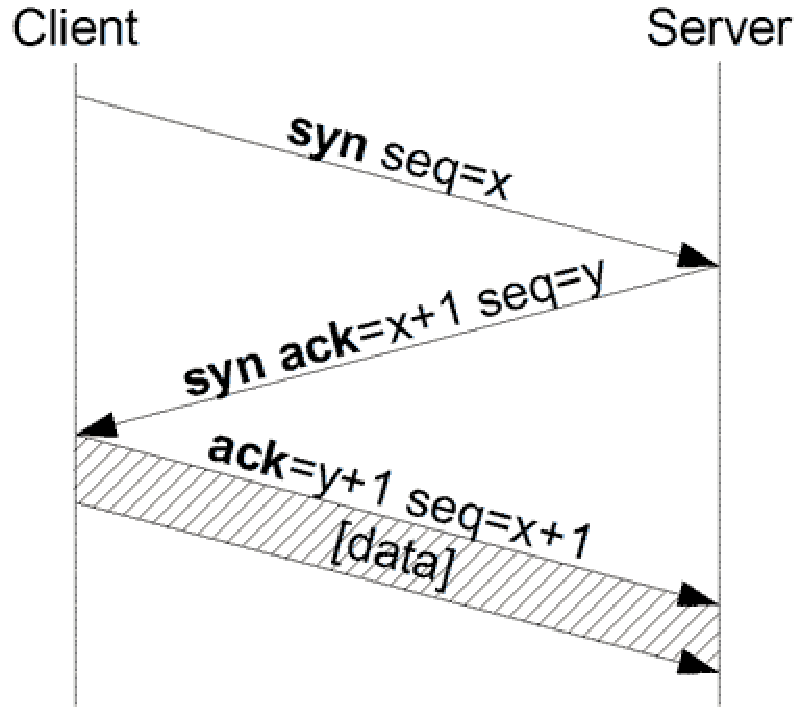
\includegraphics[width=0.3\textheight]{images/TCP_3wayhandshake.pdf}
	\caption{TCP 3-Wege-Handshake}
	\label{fig:tcp_3wayhandshake}
\end{figure}

Mithilfe von geordneten Sequenznummern und Acknowledgments werden alle empfangene Pakete bestätigt. Durch das Fehlen einer Sequenznummer erkennt der Empfänger den Verlust eines Pakets und teilt daraufhin dem Sender mit, dass es nicht angekommen ist. Für den Fall eines Verlusts des Acknowledgments, hat der Sender einen Timer, welcher nach einiger Zeit eine Retransmission des Pakets veranlasst, sofern kein Acknowledgment ankommen sollte. \\

Für die Kommunikation mit dem Roboter ist TCP aufgrund seiner höheren Übertragungszeit die ungeeignetere Variante als UDP. Auch der höhere Traffic, der vom Roboter verarbeitet werden muss könnte zu Problemen führen.


\section{HTTP}
Das Hypertext Transfer Protocol ist ein zustandsloses Datenübertragungsprotokoll, das auf der Anwendungsschicht arbeitet. Am meisten wird das Protokoll für den Aufbau von Internetseiten verwendet, also von einem Webbrowser, jedoch ist das Aufgabenfeld nicht darauf beschränkt.

HTTP arbeitet mittels zwei Befehlsarten, dem Request und dem Response. Möchte ein Browser eine Datei von einem Server laden, so sendet er einen Request mit dem Namen der Datei. \\
Einige mögliche Befehle sind: 
\begin{description}
	\item[GET] fordert eine Ressource auf dem Server an
	\item[POST] sendet Daten zur weiteren Verarbeitung zum Server
	\item[PUT] lädt eine Ressource auf den Server
	\item[DELETE] löscht eine Ressource auf dem Server (Wird kaum verwendet)
\end{description} Nachdem der Request beim Server eingegangen ist und verarbeitet wurde, sendet er einen Response. In diesem Response sind Informationen über Server und Datei enthalten, sowie die Nutzdaten, also die angefragte Datei. 


\section{AJAX}
AJAX bedeutet ausgeschrieben Asynchronous Javascript And XML und bezeichnet ein Konzept der asynchronen Datenübertragung zwischen einem Browser und einem Server mittels HTTP. Dies ermöglicht die Veränderung der im Browser geladenen Seite, auch wenn der Server noch nicht geantwortet hat. \\
Generell wäre AJAX ein Ansatz mit dem man die Kommunikation zwischen Webanwendung und Server realisieren könnte, jedoch hat es den Nachteil, dass pro Aufruf eine extra Verbindung aufgebaut wird. Bei häufigen Aufrufen könnte dies zu Problemen führen. Ein weiterer Nachteil ist, dass der eigentliche Sendevorgang vom Client über den Server geregelt wird, wodurch es nicht ohne weiteres möglich wäre, den Absender zu identifizieren. Der größte Nachteil wäre jedoch, dass für diese Art von Kommunikation eine eigene Schnittstelle für Webanwendung und eine für die Android-Anwendung zur Verfügung stehen muss. Mit anderen Protokollen (siehe \ref{sec:websockets}) ist genau das möglich.


\section{WebSockets}
\label{sec:websockets}
Das WebSocket-Protokoll ist ein Netzwerkprotokoll, das auf TCP und HTTP basiert. In diesem Protokoll ist es möglich, eine bidirektionale Verbindung zwischen einer Webanwendung und einem WebSocket-Server herzustellen. Im Gegensatz zu reinem HTTP ist es hierbei möglich, dass der Server ohne einen vorhergehenden Request des Clients, Daten an den Client sendet. Lediglich den Verbindungsaufbau muss der Client initiieren. Dies wird realisiert, indem die TCP-Verbindung nach dem Verbindungsaufbau nicht sofort geschlossen wird. 
Eine WebSocket URL wird über die beiden Schemata wss und ws definiert, was für verschlüsselte und unverschlüsselte Verbindungen steht.

Der Verbindungsaufbau funktioniert über einen Handshake, der wie in HTTP üblich über einen Request und anschließenden Response erreicht wird. Aufgrund der Tatsache, dass die HTTP-Header nur beim Verbindungsaufbau gesendet werden und dadurch der Traffic durch den HTTP-Header gering ist, wird das Protokoll hauptsächlich von Anwendungen verwendet, die regelmäßige Kommunikation zwischen Client und Server verlangen, wie zum Beispiel Online-Spiele. \\

Für die Kommunikation mit den Steuergeräten stellen die WebSockets eine praktische Lösung dar. Da als Grundlage TCP für die WebSockets verwendet werden ist es möglich eine dauerhafte Verbindung zu halten. Vor allem die Webanwendung schränkt die Übertragungsprotokolle enorm ein, da es Client-Seitig nicht möglich ist eine direkte TCP Verbindung aufzubauen, HTTP jedoch schon. Mit WebSockets ist es möglich eine einheitliche Schnittstelle für die Steuergeräte zu erstellen, unabhängig von welcher Plattform sie zugreifen.



\section{Jetty Webserver}
Jetty \cite{JETTY} ist eine Java-Implementierung eines Webservers. Durch seine geringe Größe ist es leicht, ihn in andere Software zu integrieren. Außerdem unterstützt Jetty die Möglichkeit WebSockets aufzubauen. Damit ist Jetty eine gute Wahl, um die Webanwendung zusammen mit der anderen Software bereitzustellen, ohne einen extra Webserver zu konfigurieren.



\section{Base64}
Base64 ist ein Kodierungsverfahren, bei dem 8-Bit Binärdaten in eine rein aus lesbaren Zeichen bestehende Zeichenkette umgewandelt wird. Bei diesem verfahren steigt der benötigte Platzbedarf um 33-36 \%. Jedoch ist es für eine sehr Hardware-abstrahierte Programmiersprache wie Javascript ungeeignet auf Byte-Ebene zu kommunizieren. Mit der base64 Kodierung wird eine reine Zeichen basierte Übertragung mit den Steuergeräten möglich.

\section{Der Roboter}
Wie schon erwähnt wurde der Roboter im Rahmen einer weiteren Bachelorarbeit erstellt. Hier soll nur kurz auf die für diese Arbeit wichtigen Aspekte des Roboters eingegangen werden. \\
Der Roboter verfügt über zwei Räder, die über jeweils einen Motor beschleunigt und abgebremst werden können. Außerdem befindet sich vorne ein Schussmechanismus, der mit einem Befehl (vgl. \ref{sec:schnittstelle}) ausgelöst werden kann. Die beiden Motoren der Räder beschleunigen den Roboter auf bis zu $2\frac{m}{s}$. Dadurch wird ersichtlich, dass bei hohen Geschwindigkeiten eine gute Reaktionszeit notwendig ist, damit sich der Roboter noch steuern lässt.